\documentclass[letterpaper,11pt]{article}

\usepackage{latexsym}
\usepackage[empty]{fullpage}
\usepackage{titlesec}
\usepackage{marvosym}
\usepackage[usenames,dvipsnames]{color}
\usepackage{verbatim}
\usepackage{enumitem}
\usepackage[hidelinks]{hyperref}
\usepackage{fancyhdr}
\usepackage[english]{babel}
\usepackage{tabularx}
\usepackage{fontawesome5}
\usepackage{multicol}
\setlength{\multicolsep}{-3.0pt}
\setlength{\columnsep}{-1pt}
\input{glyphtounicode}

%new packages

\usepackage{fontenc}
\usepackage{amsmath}
\usepackage{amssymb}
\usepackage{graphicx}



%----------FONT OPTIONS----------

\pagestyle{fancy}
\fancyhf{} % clear all header and footer fields
\fancyfoot{}
\renewcommand{\headrulewidth}{0pt}
\renewcommand{\footrulewidth}{0pt}

% Adjust margins
\addtolength{\oddsidemargin}{-0.6in}
\addtolength{\evensidemargin}{-0.5in}
\addtolength{\textwidth}{1.19in}
\addtolength{\topmargin}{-.7in}
\addtolength{\textheight}{1.4in}

\urlstyle{same}

\raggedbottom
\raggedright
\setlength{\tabcolsep}{0in}

% Sections formatting
\titleformat{\section}{
  \vspace{-4pt}\scshape\raggedright\large\bfseries
}{}{0em}{}[\color{black}\titlerule \vspace{-5pt}]



% Ensure that generate pdf is machine readable/ATS parsable
\pdfgentounicode=1

%-------------------------
% Custom commands
\newcommand{\resumeItem}[1]{
  \item\small{
    {#1 \vspace{-2pt}}
  }
}

\newcommand{\classesList}[4]{
    \item\small{
        {#1 #2 #3 #4 \vspace{-2pt}}
  }
}

\newcommand{\resumeSubheading}[4]{
  \vspace{-2pt}\item
    \begin{tabular*}{1.0\textwidth}[t]{l@{\extracolsep{\fill}}r}
      \textbf{#1} & \textbf{\small #2} \\
      \textit{\small#3} & \textit{\small #4} \\
    \end{tabular*}\vspace{-7pt}
}

\newcommand{\resumeSubSubheading}[2]{
    \item
    \begin{tabular*}{0.97\textwidth}{l@{\extracolsep{\fill}}r}
      \textit{\small#1} & \textit{\small #2} \\
    \end{tabular*}\vspace{-7pt}
}

\newcommand{\resumeProjectHeading}[2]{
    \item
    \begin{tabular*}{1.001\textwidth}{l@{\extracolsep{\fill}}r}
      \small#1 & \textbf{\small #2}\\
    \end{tabular*}\vspace{-7pt}
}


\newcommand{\resumeSubItem}[1]{\resumeItem{#1}\vspace{-4pt}}

\renewcommand\labelitemi{$\vcenter{\hbox{\tiny$\bullet$}}$}
\renewcommand\labelitemii{$\vcenter{\hbox{\tiny$\bullet$}}$}

\newcommand{\resumeSubHeadingListStart}{\begin{itemize}[leftmargin=0.0in, label={}]}
\newcommand{\resumeSubHeadingListEnd}{\end{itemize}}
\newcommand{\resumeItemListStart}{\begin{itemize}}
\newcommand{\resumeItemListEnd}{\end{itemize}\vspace{-5pt}}

\begin{document}
\fontfamily{cmr}\selectfont
\begin{center}
\parbox{3.0cm}{%
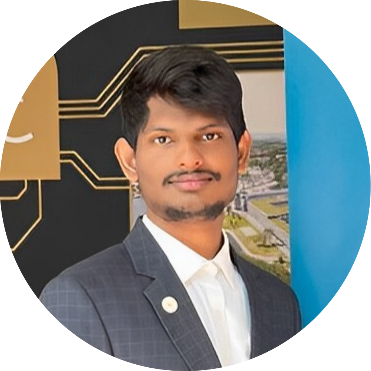
\includegraphics[width=2.7cm,clip]{images/resume_pic_m.png}}
\parbox{\dimexpr\linewidth-3.8cm\relax}{
\vspace{-20pt}
\begin{tabularx}{\linewidth}{L r} \\
    {\Huge \scshape  Venkata Sai Yakkshit Reddy Asodi}~
    \href{https://www.cedzlabs.com/yakkshit}{\vspace{1pt}}\\
      Berlin, Germany. \\ \vspace{1pt}
     \small \raisebox{-0.1\height}\faPhone\ +91 9493006444 ~ \href{mailto:saiyakkshit2001@gmail.com}{\raisebox{-0.2\height}\faEnvelope\  {saiyakkshit2001@gmail.com}} ~ 
    \href{https://linkedin.com/in/yakkshit/}{\raisebox{-0.2\height}\faLinkedin\ {yakkshit}}  ~
    \href{https://yakkshit.com/}{\raisebox{-0.2\height}\faGlobe\ {yakkshit.com}}  ~
    \href{https://github.com/yakkshit}{\raisebox{-0.2\height}\faGithub{ yakkshit}}
    \vspace{-8pt}
\end{tabularx}
}
\end{center}

\vspace{-23pt}
%-----------SUMMARY-----------
\section{Summary \faLink}
Full-stack developer with extensive experience in TypeScript, React, and Java-based microservices architecture. Proven track record in developing scalable enterprise applications with a focus on clean code and test-driven development. Passionate about exploring new technologies and implementing efficient solutions for complex business requirements. Experienced in agile methodologies and continuous deployment practices.

%-----------TECHNICAL SKILLS-----------
\section{\href{https://www.linkedin.com/in/yakkshit/details/skills/}{Technical Skills} \faLink}
\begin{itemize}[leftmargin=0.15in, label={}]
\small{\item{
\textbf{Languages - }{TypeScript, Java, Kotlin, JavaScript} \\
\textbf{Frontend - }{React, Tailwind CSS, HTML5, CSS3} \\
\textbf{Backend - }{Spring Boot, RESTful APIs, Microservices} \\
\textbf{Cloud \& DevOps - }{Azure, Docker, Kubernetes, CI/CD} \\
\textbf{Testing \& Tools - }{Jest, JUnit, Gradle, Git}
}}
\end{itemize}
\vspace{-10pt}

%-----------EXPERIENCE-----------
\section{Experience \faLinkedin}

\resumeSubHeadingListStart

\resumeSubheading
{\large Circleup AG \faBuilding}{December 2023 -- July 2024}
{Lead Full Stack Engineer}{\faMapMarker \hspace{0.1cm} Zurich, Switzerland}\\
\vspace{10pt}
\textbf{Responsibilities:}
\resumeItemListStart
\vspace{-10pt}
\resumeItem{Architected and implemented microservices using Spring Boot and Kotlin, ensuring high performance and scalability.}
\resumeItem{Developed modern frontend applications using TypeScript and React, implementing clean architecture patterns.}
\resumeItem{Led the migration from monolithic to microservices architecture, improving system reliability and maintainability.}
\resumeItemListEnd
\vspace{-3pt}
\textbf{Environment:}\emph{TypeScript, React, Java, Spring Boot, Azure, Gradle}

\resumeSubheading
{Cedzlabs \faBuilding}{March 2023 -- July 2024}
{Full Stack Engineer}{\faMapMarker \hspace{0.1cm} Berlin, Germany}\\
\vspace{10pt}
\textbf{Responsibilities:}
\vspace{-10pt}
\resumeItemListStart
\resumeItem{Built and maintained RESTful APIs using Java and Spring Boot, following test-driven development practices.}
\resumeItem{Implemented responsive UI components using React and Tailwind CSS, ensuring optimal user experience.}
\resumeItemListEnd
\vspace{-3pt}
\textbf{Environment:}\emph{TypeScript, React, Java, Spring Boot, Azure}

%-----------PROJECTS-----------
\section{Projects \faGithub}
\vspace{-5pt}
\resumeSubHeadingListStart
\resumeProjectHeading
{\textbf{\href{https://ui.cedzlabs.com/resume}{Enterprise Resource Management System}} $|$ \emph{TypeScript, Spring Boot}}{2023}\\
\vspace{6pt}
\textbf{Description:}
\vspace{-5pt}
\resumeItemListStart
\resumeItem{Developed a comprehensive resource management system using TypeScript and Spring Boot microservices. Implemented clean architecture patterns and automated testing, achieving 95\% test coverage. Integrated with Azure cloud services for scalability and deployed using CI/CD pipelines.}
\resumeItemListEnd
\vspace{4pt}
\textbf{Tools:}\emph{TypeScript, React, Java, Spring Boot, Azure, Gradle}
\vspace{-10pt}

\resumeProjectHeading
{\href{https://yakkshit.com}{\textbf{Financial Data Processing Platform}} $|$ \emph{Kotlin, React}}{2023}\\
\vspace{6pt}
\textbf{Description:}
\vspace{-5pt}
\resumeItemListStart
\resumeItem{Built a scalable financial data processing platform using Kotlin microservices and React frontend. Implemented automated testing and continuous deployment using Azure DevOps. Reduced data processing time by 60\% through efficient microservice architecture.}
\resumeItemListEnd
\vspace{4pt}
\textbf{Tools:}\emph{Kotlin, React, TypeScript, Azure, Gradle}
\vspace{-12pt}

%-----------ACHIEVEMENTS---------------
\section{Achievements / Certifications}
\resumeSubHeadingListStart
\resumeItemListStart
\resumeItem{Implemented microservices architecture that reduced system response time by 40\%.}
\resumeItem{Azure Certified Developer with expertise in cloud-native applications.}
\resumeItem{Led successful migration of legacy systems to modern TypeScript/React stack.}
\resumeItemListEnd

\resumeSubHeadingListEnd
\textbf{Strengths:}\emph{Clean code, microservices architecture, test-driven development, agile methodologies} \\
\textbf{Languages:}\emph{Telugu - Native $|$ English - Fluent $|$ Hindi - Fluent $|$ German - Elementary $|$ Swedish - Elementary}

\vspace{10pt}
\end{document}